\chapter{Tests and examples}

@O test/jl/runtests.jl
@{using LARLIB

include("./planar_arrangement.jl")
include("./dimension_travel.jl")
include("./utilities.jl")
@}

@O examples/jl/general_tests.jl
@{using LARLIB

@< planar\_arrangement tests @>
@< spatial\_arrangement tests @>
@}

%%%%%%%%%%%%%%%%%%%%%%%
\section{Planar arrangement tests}
\label{ch:planar_arrangement_tests}

Here we present some general tests for the \texttt{planar\_arrangement} function [ref. \ref{ch:planar_arrangement}]

@D planar\_arrangement tests
@{function generate_perpendicular_lines(steps::Int, minlen, maxlen)
    V = zeros(0,2)

    function rec(o, d, s)
        if s == 0 return end

        a = (maxlen-minlen)*rand() + minlen
        p = o + a*d
        V = [V; o; p]

        b = (a-minlen)*rand() + minlen
        p = o + b*d
        rec(p, d, s-1)

        b = (a-minlen)*rand() + minlen
        p = o + b*d
        rec(p, perpendicular(d), s-1)
    end

    function perpendicular(vec)
        v = zeros(size(vec))
        v[1] = vec[2]
        v[2] = vec[1]
        return v
    end

    rec([0 0], [1 0], steps)
    rec([0 0], [0 1], steps)
    vnum = size(V, 1)
    enum = vnum >> 1
    EV = spzeros(Int8, enum, vnum)
    for i in 1:enum
        EV[i, i*2-1:i*2] = 1
    end
    V, EV
end


function generate_random_lines(n, points_range, alphas_range)
    origins = points_range[1] + (points_range[2]-points_range[1])*rand(n, 2)
    directions = mapslices(normalize, rand(n, 2) - .5*ones(n, 2), 2)
    alphas = alphas_range[1] + (alphas_range[2]-alphas_range[1])*rand(n)
    new_points = Array{Float64, 2}(n, 2)
    for i in 1:n
        new_points[i, :] = origins[i, :] + alphas[i]*directions[i, :]
    end
    V = [origins; new_points]
    EV = spzeros(Int8, n, n*2)
    for i in 1:n
        EV[i, i] = 1
        EV[i, n+i] = 1
    end
    V, EV
end
@}

\vfill

\begin{figure}[p!]
    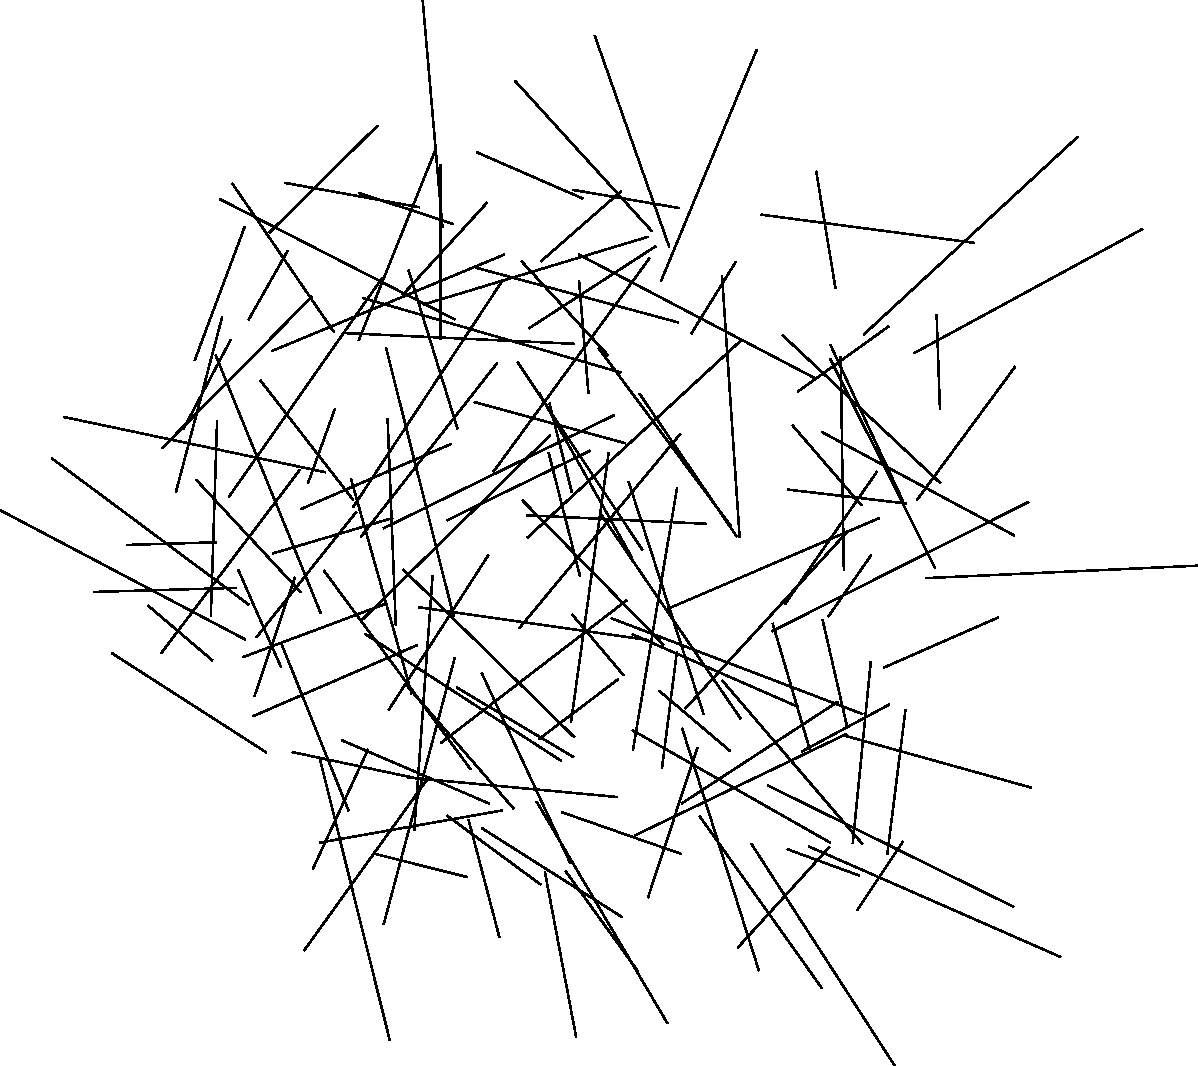
\includegraphics[width=\textwidth]{./img/test-lines.pdf}%
    \caption{Input}
\end{figure}


\begin{figure}[p!]
    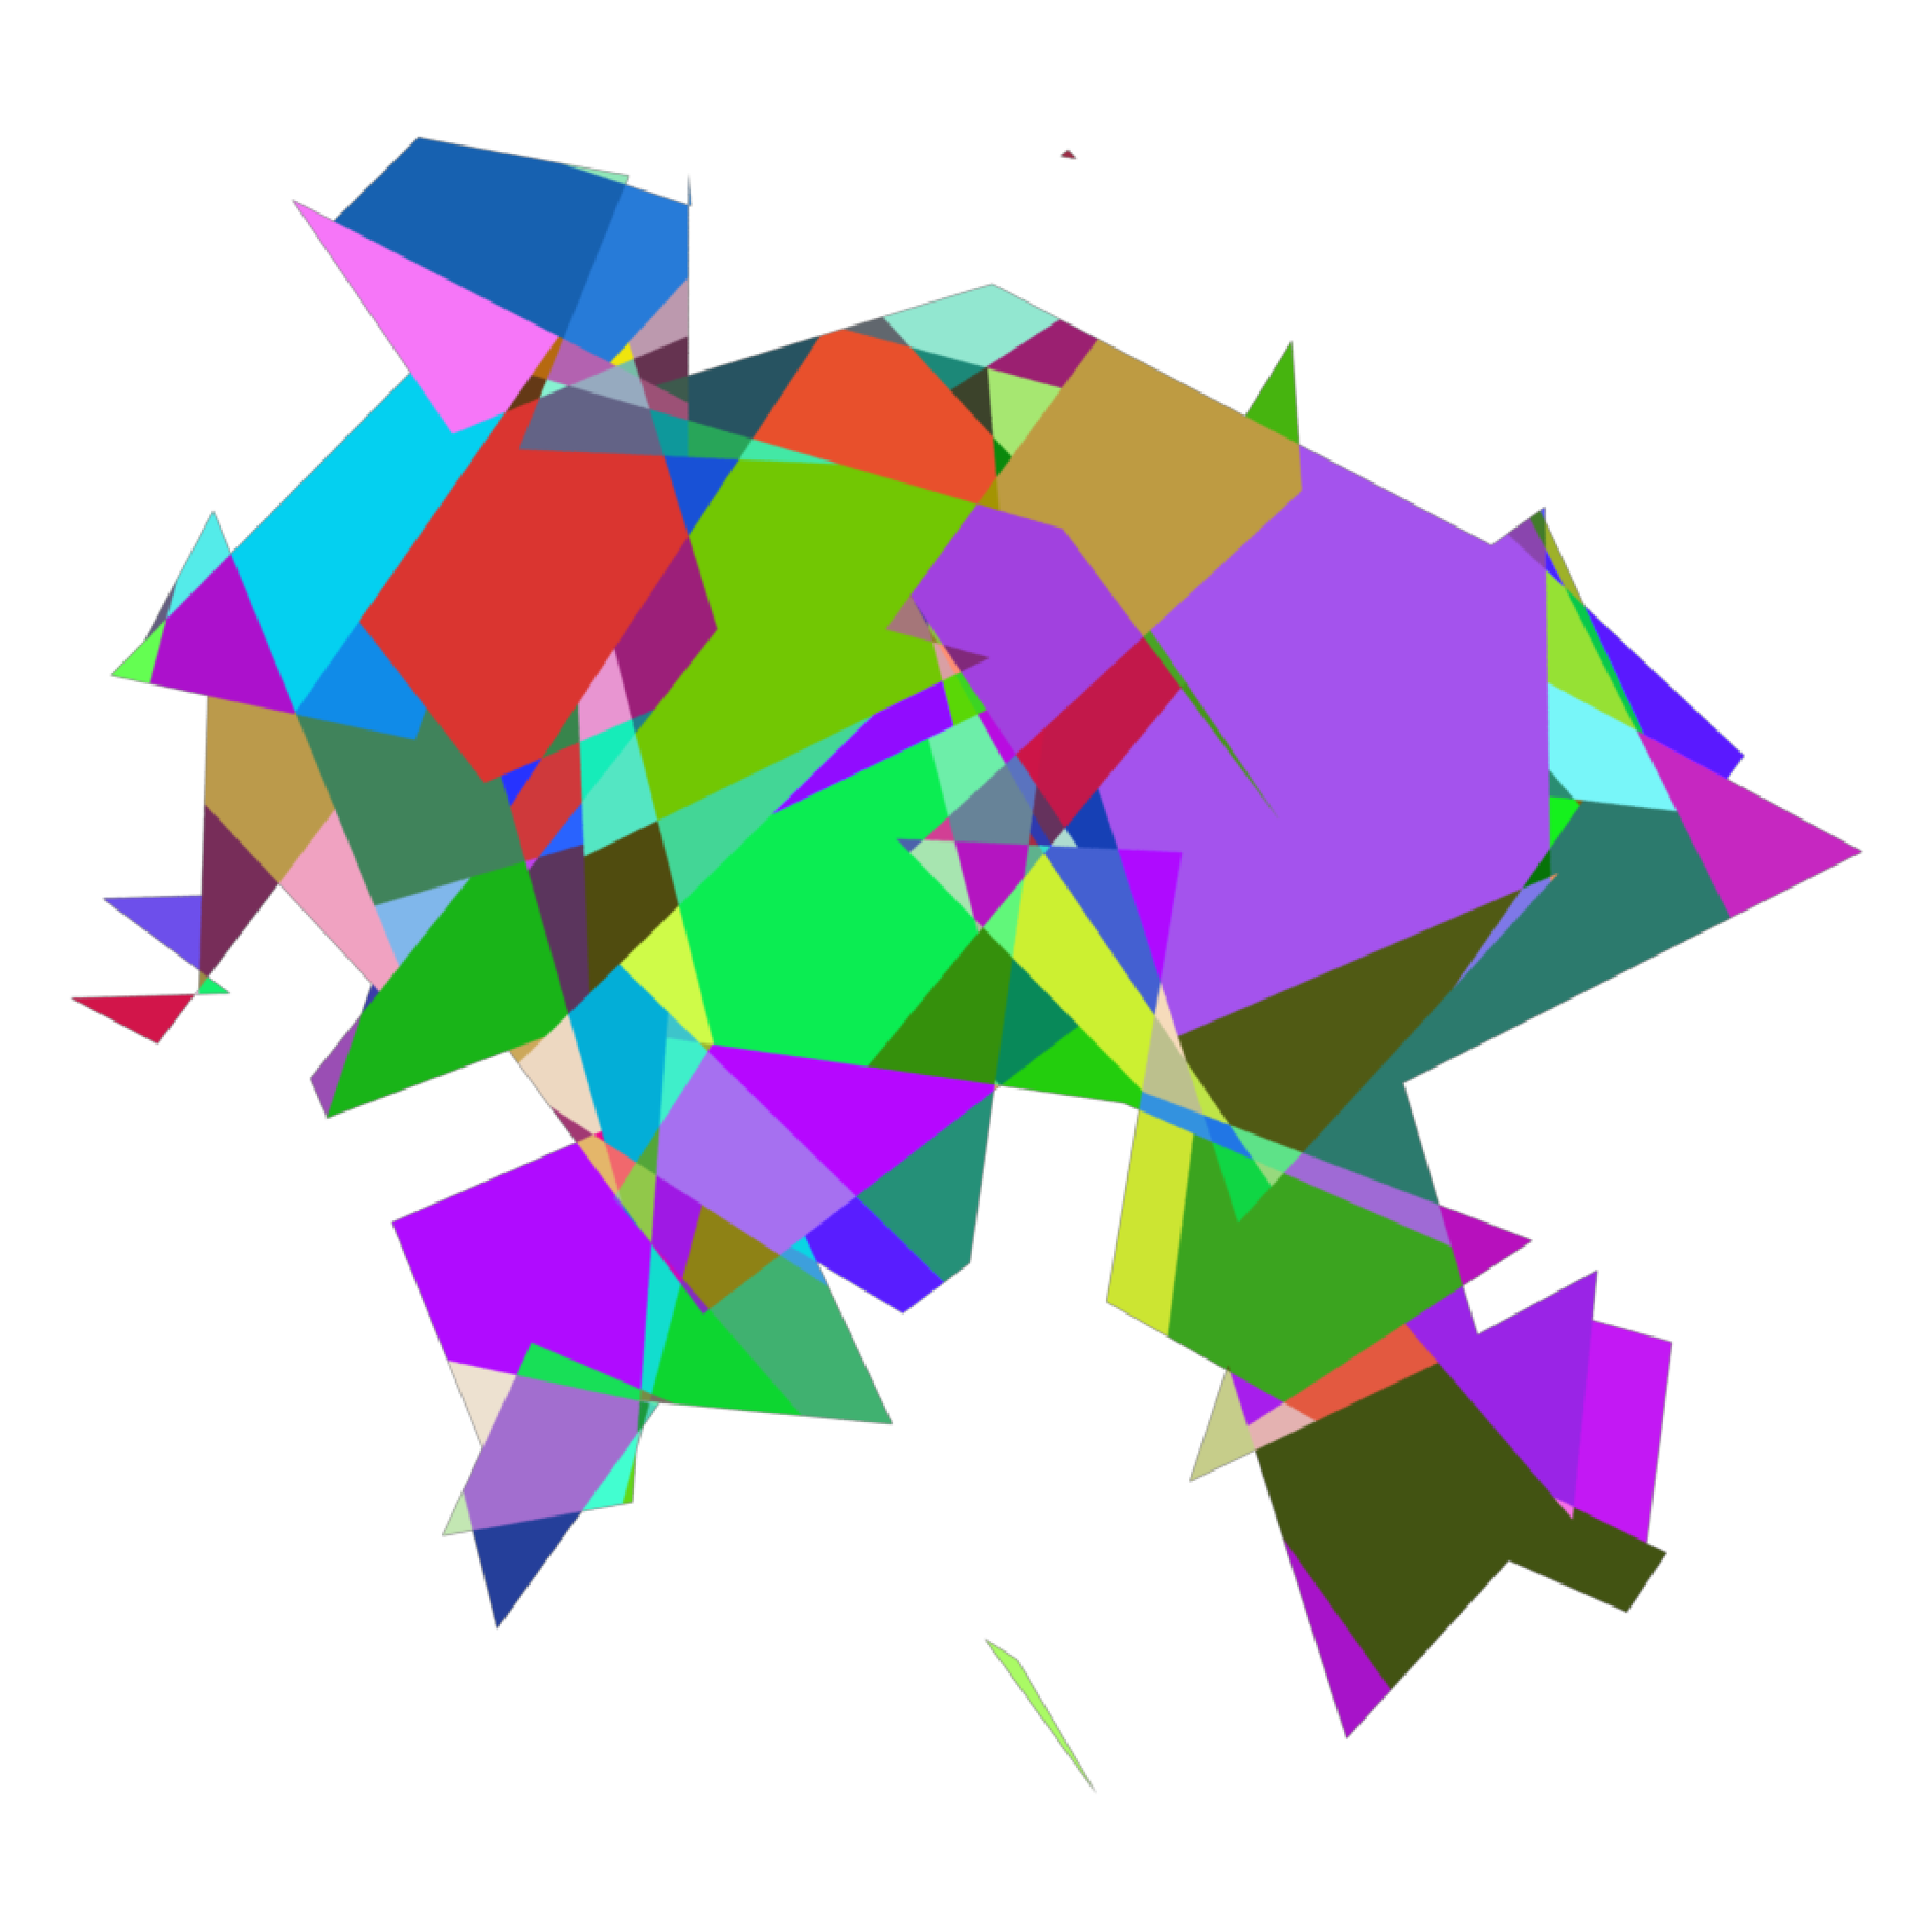
\includegraphics[width=\textwidth]{./img/test-lines-out-compact.pdf}%
    \caption{Output}
\end{figure}

\begin{figure}[p!]
    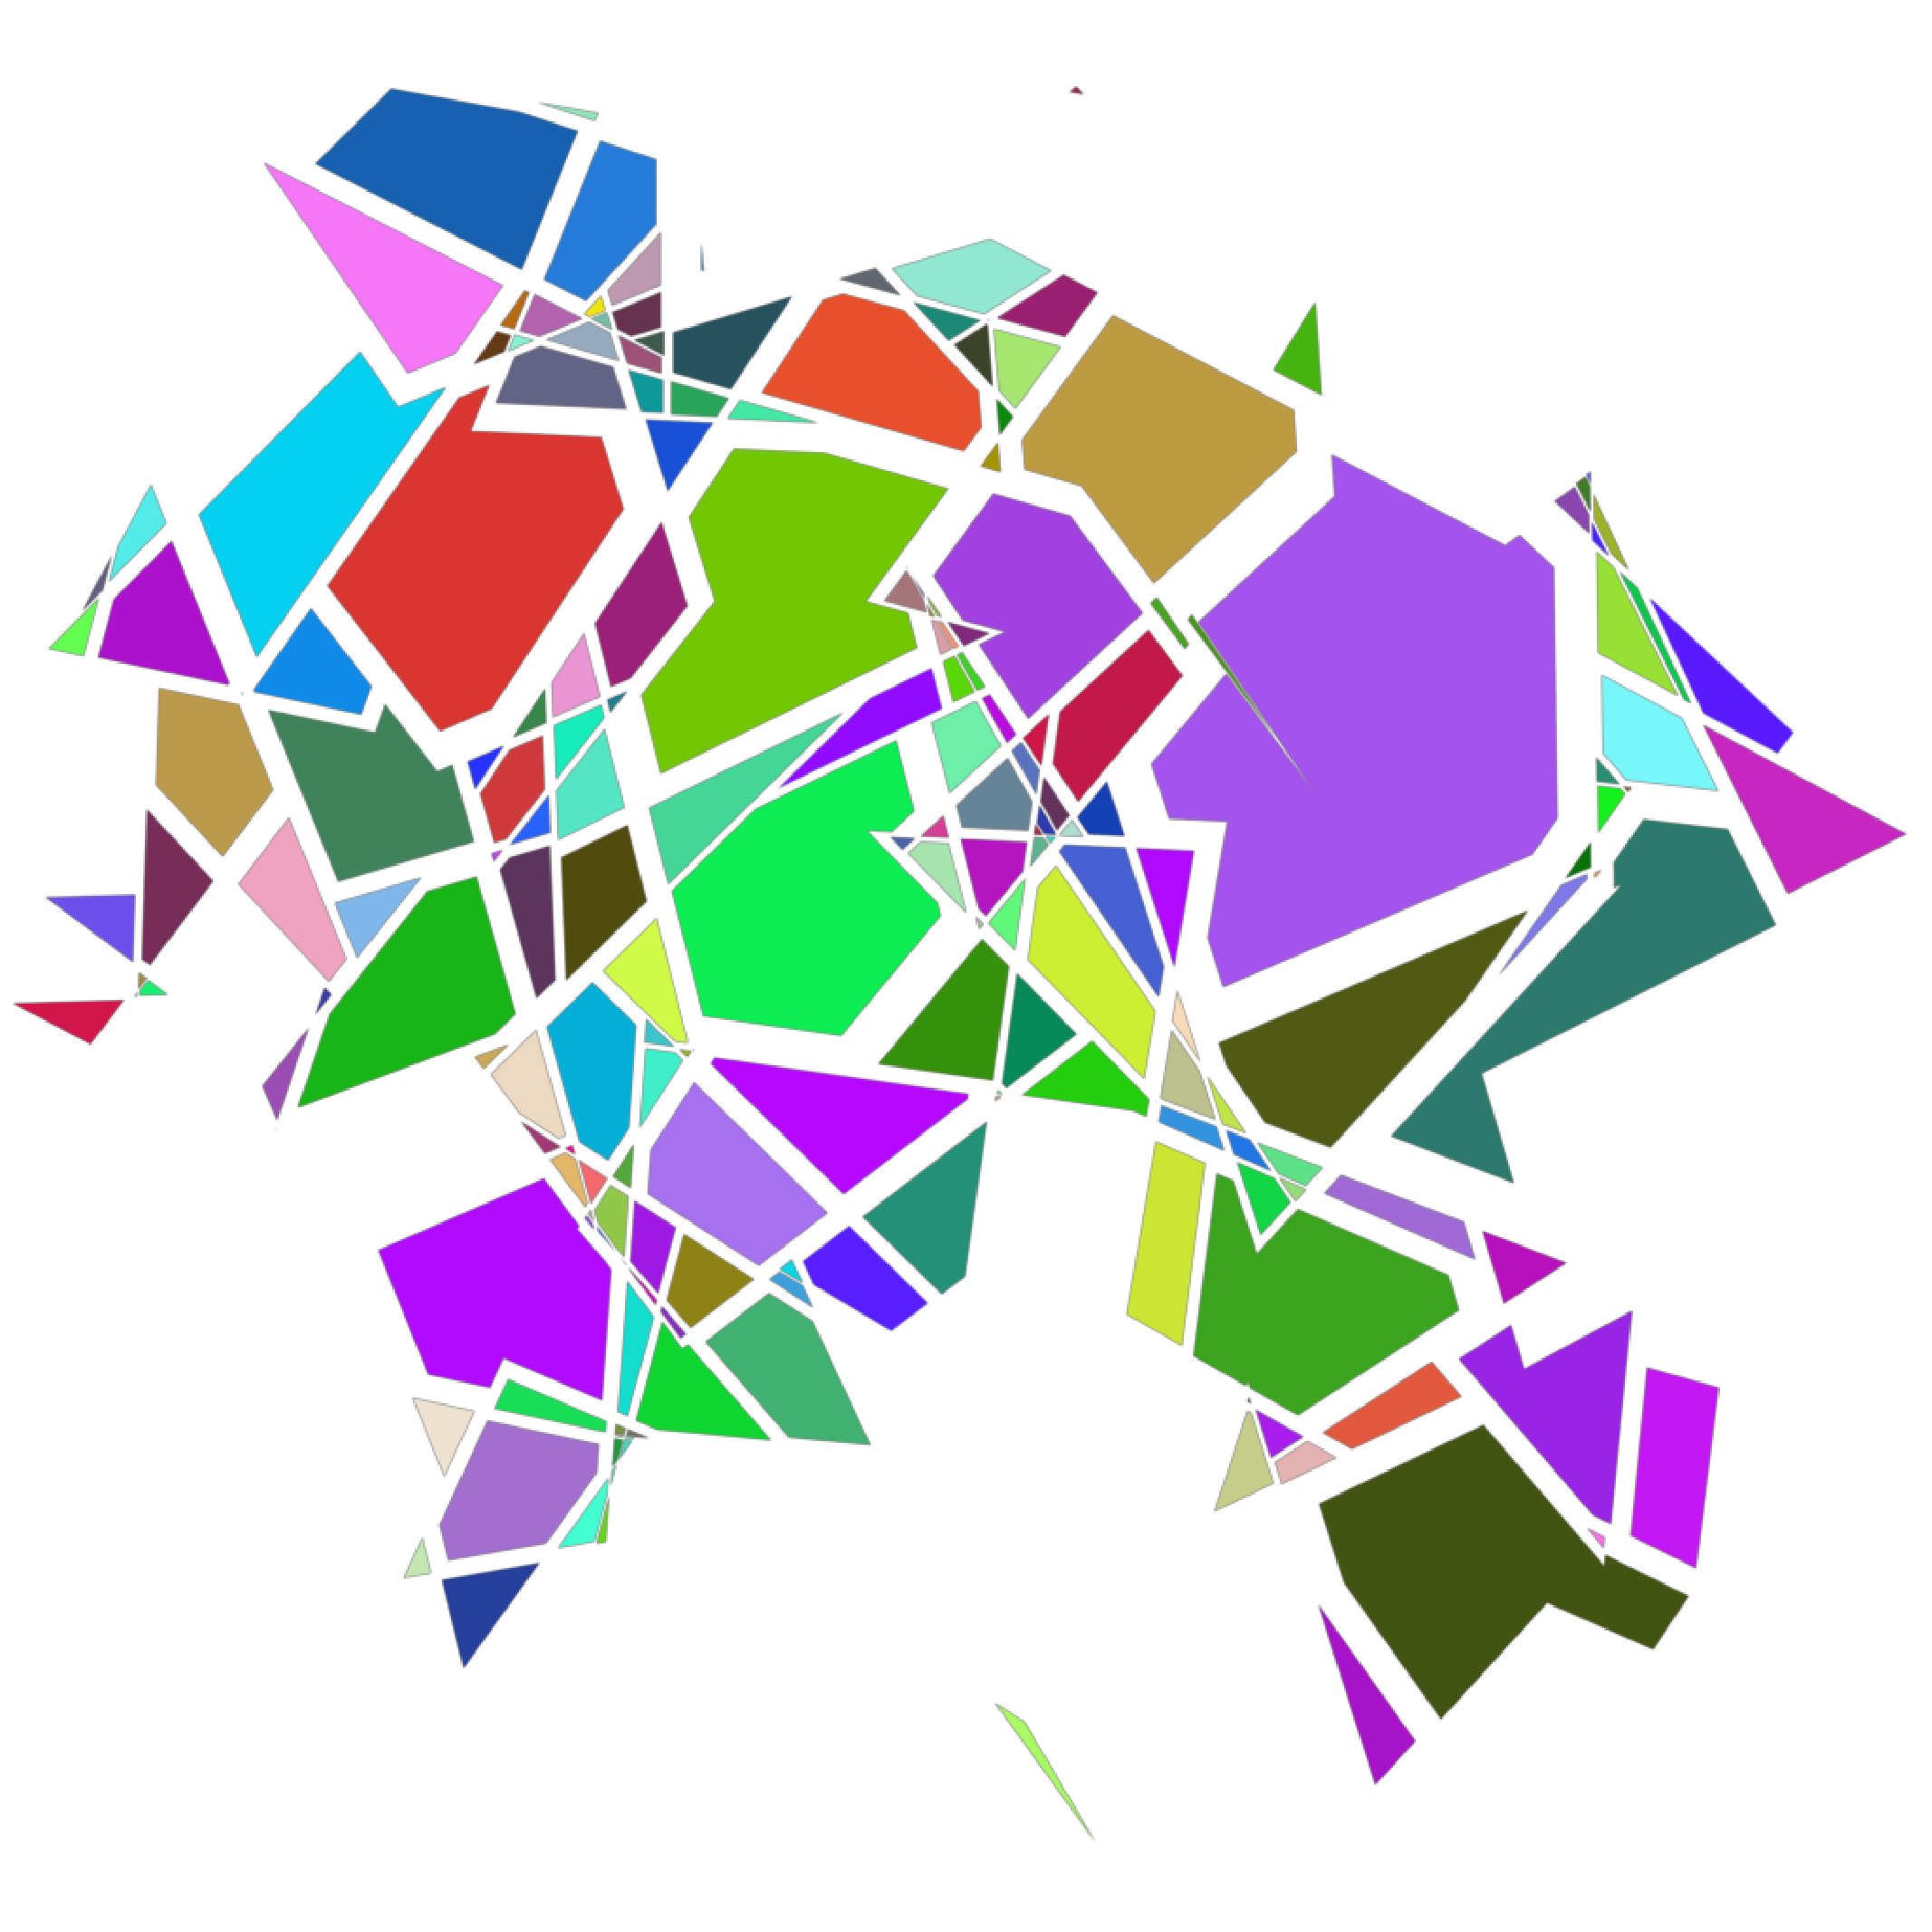
\includegraphics[width=\textwidth]{./img/test-lines-out.pdf}%
    \caption{Output (Exploded)}
\end{figure}

%%%%%%%%%%%%%%%%%%%%%%%
\section{Spatial arrangement tests}
\label{ch:spatial_arrangement_tests}

We used this test a lot during development. It builds
a cube made of $3 \times 3 \times 3$ cubes. The it arranges
the cubes, building a sort of Rubik's cube. Then it duplicates
it and rotates a copy by $\pi / 6$ on the $x_1$-axis
and then on the $x_3$-axis.

@D spatial\_arrangement tests
@{function rubiks_example(ncubes = 3)
    V = Float64[
        0 0 0; 0 1 0;
        1 1 0; 1 0 0;
        0 0 1; 0 1 1;
        1 1 1; 1 0 1
    ]

    EV = sparse(Int8[
        -1  1  0  0  0  0  0  0;
        0 -1  1  0  0  0  0  0;
        0  0 -1  1  0  0  0  0;
        -1  0  0  1  0  0  0  0;
        -1  0  0  0  1  0  0  0;
        0 -1  0  0  0  1  0  0;
        0  0 -1  0  0  0  1  0;
        0  0  0 -1  0  0  0  1;
        0  0  0  0 -1  1  0  0;
        0  0  0  0  0 -1  1  0;
        0  0  0  0  0  0 -1  1;
        0  0  0  0 -1  0  0  1;
    ])

    FE = sparse(Int8[
        1  1  1 -1  0  0  0  0  0  0  0  0;
        0  0  0  0  0  0  0  0 -1 -1 -1  1;
        -1  0  0  0  1 -1  0  0  1  0  0  0;
        0 -1  0  0  0  1 -1  0  0  1  0  0;
        0  0 -1  0  0  0  1 -1  0  0  1  0;
        0  0  0  1 -1  0  0  1  0  0  0 -1;
    ])

    cube = [V, EV, FE]
    cubesRow = (zeros(0,3),spzeros(Int8,0,0),spzeros(Int8,0,0))

    for i in 1:ncubes
        cubesRow = LARLIB.skel_merge(cubesRow..., cube...)
        cube[1] = cube[1] + [zeros(8) zeros(8) ones(8)]
    end

    cubesRow = collect(cubesRow)
    cubesPlane = cubesRow
    num = size(cubesRow[1], 1)
    for i in 1:ncubes
        cubesPlane = LARLIB.skel_merge(cubesPlane..., cubesRow...)
        cubesRow[1] = cubesRow[1] + [zeros(num) ones(num) zeros(num)]
    end

    cubesPlane = collect(cubesPlane)
    cubesCube = cubesPlane
    num = size(cubesPlane[1], 1)
    for i in 1:ncubes
        cubesCube = LARLIB.skel_merge(cubesCube..., cubesPlane...)
        cubesPlane[1] = cubesPlane[1] + [ones(num) zeros(num) zeros(num)]
    end

    println("Arranging a cube of ", ncubes^3," cubes...")
    rubik = LARLIB.spatial_arrangement(cubesCube...)
    println("DONE")

    rubik = rubik[1] - (.5*ncubes), rubik[2:3]...
    c = cos(pi/6); s = sin(pi/6)
    M1 = [1  0 0; 0 c -s; 0 s c]
    M2 = [c -s 0; s c  0; 0 0 1]
    rot_rubik = rubik[1]*M1*M2, rubik[2:3]...

    println("Arranging two rubik cubes...")
    two_rubiks = LARLIB.skel_merge(rubik..., rot_rubik...)
    println("DONE")

    arranged_rubiks = LARLIB.spatial_arrangement(two_rubiks...)
end
@}

On the next pages the results are visualized.
\begin{figure}[h]
    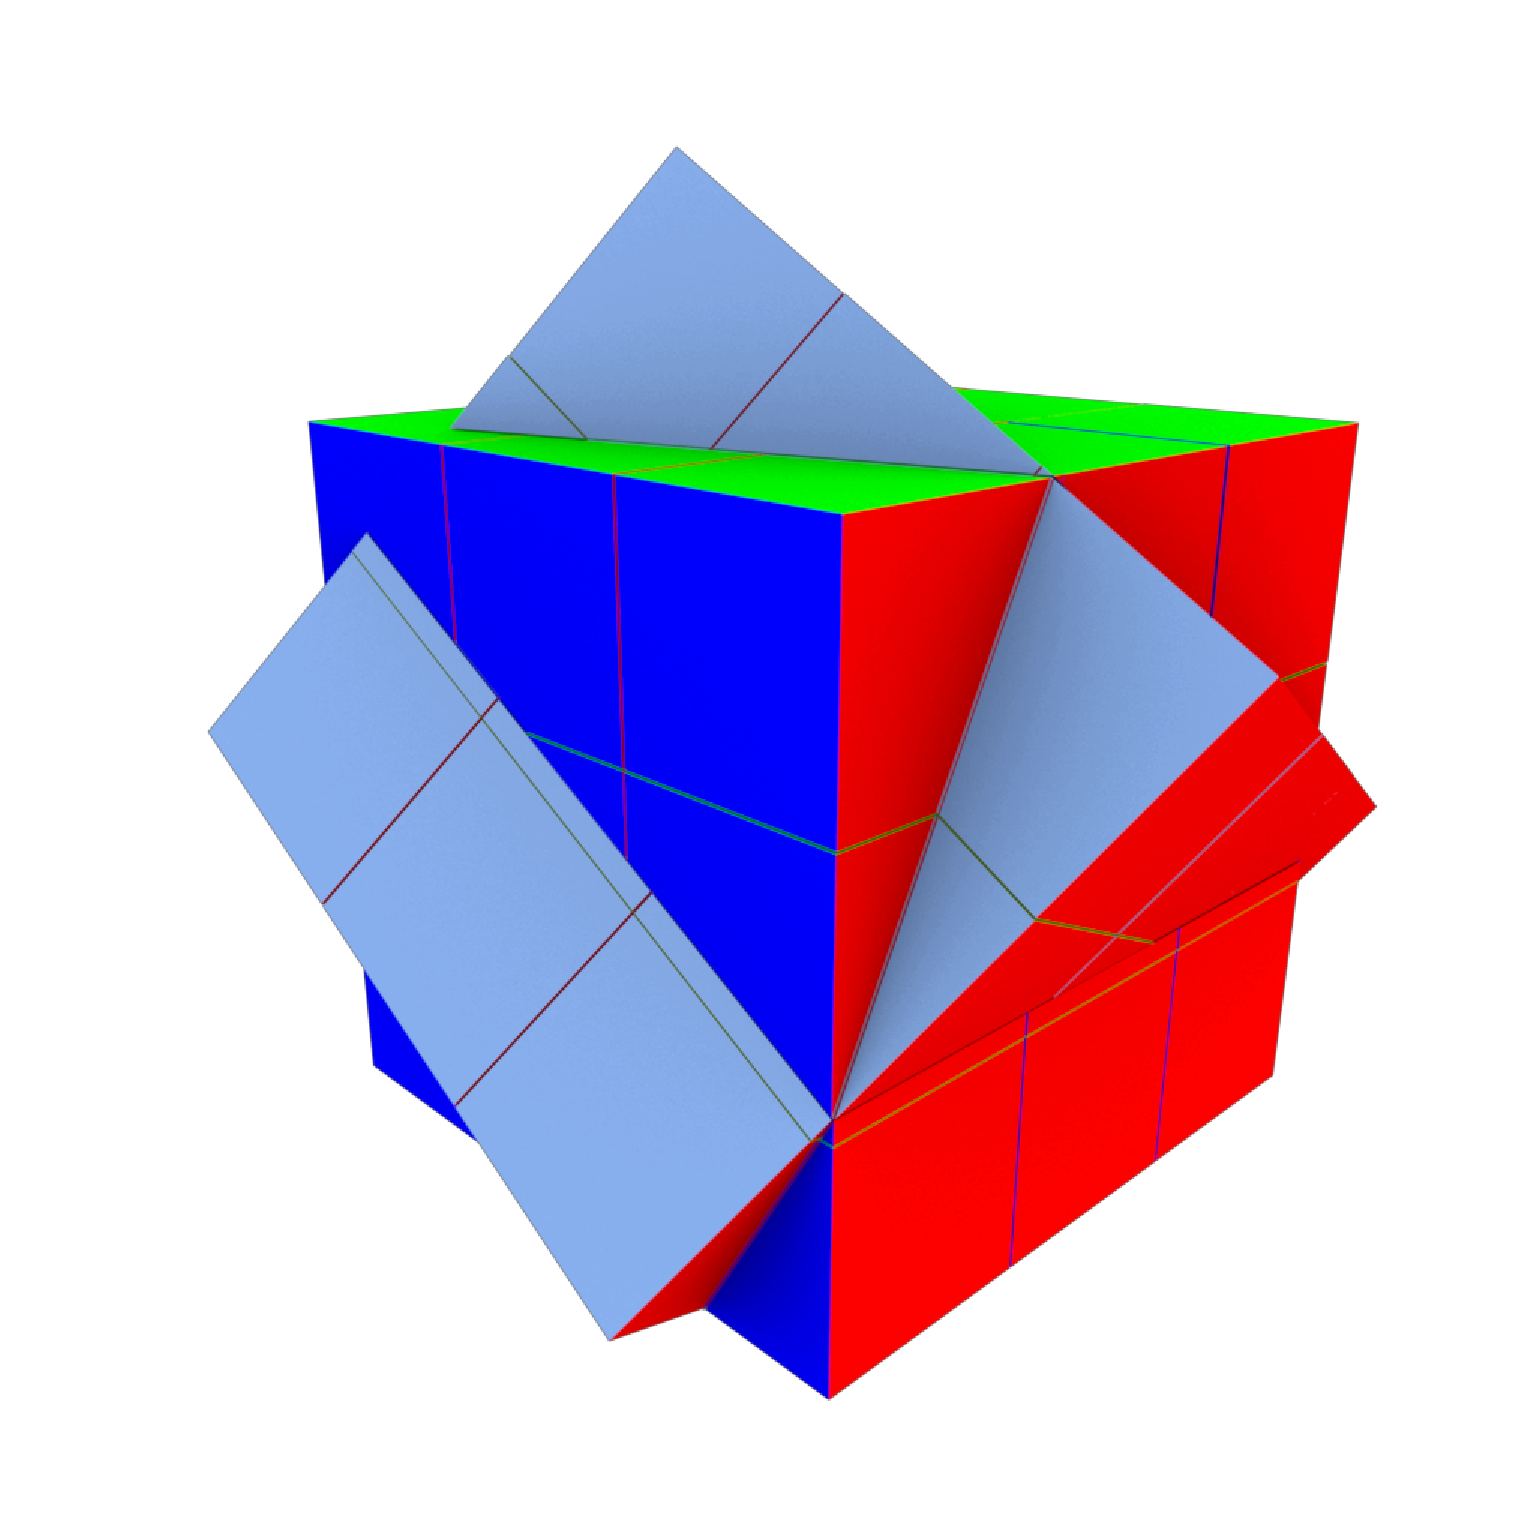
\includegraphics[width=\textwidth]{./img/test-0.pdf}%
    \caption{Input}
\end{figure}

\begin{figure}[h]
    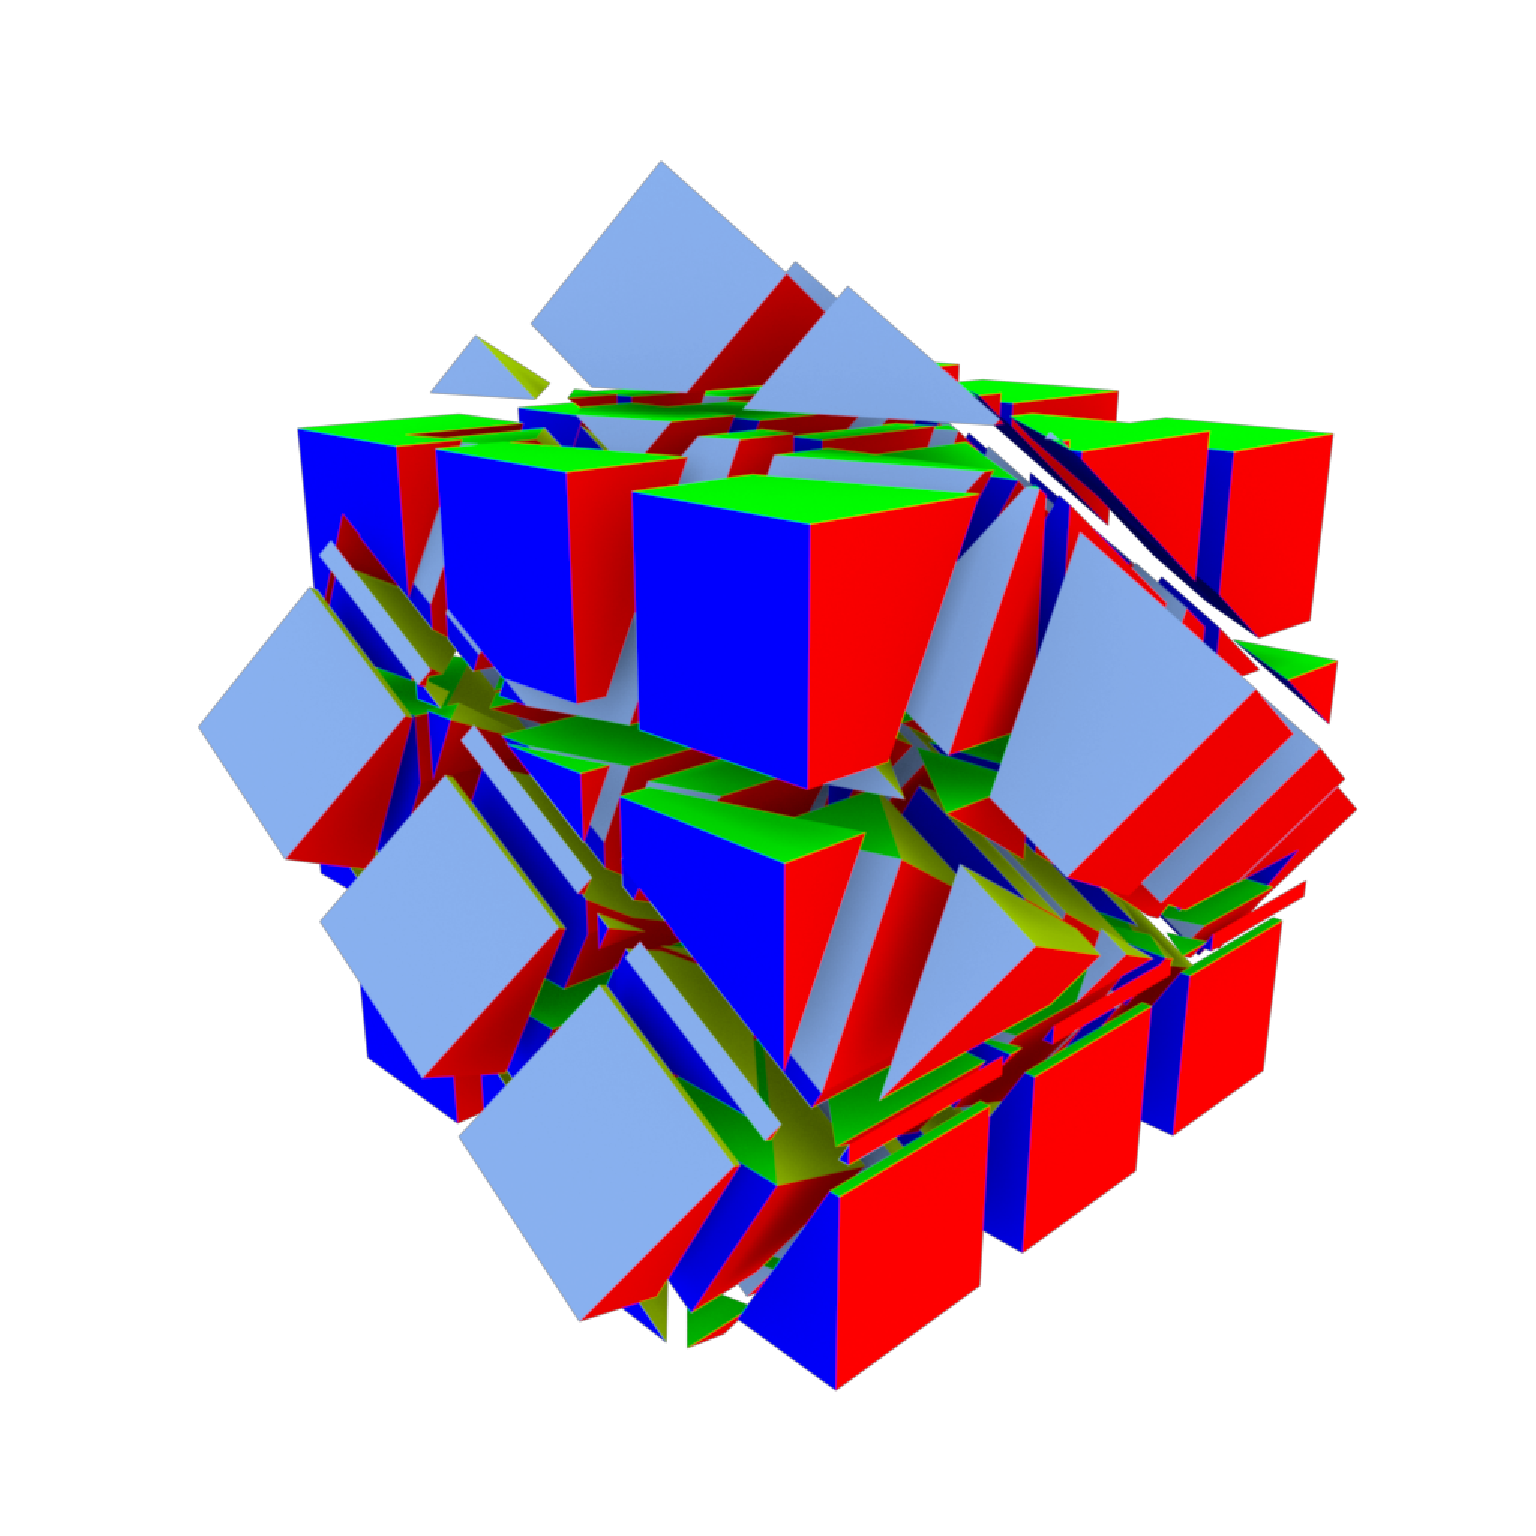
\includegraphics[width=\textwidth]{./img/test-1.pdf}%
    \caption{Output (Exploded)}
\end{figure}

\begin{figure}[h]
    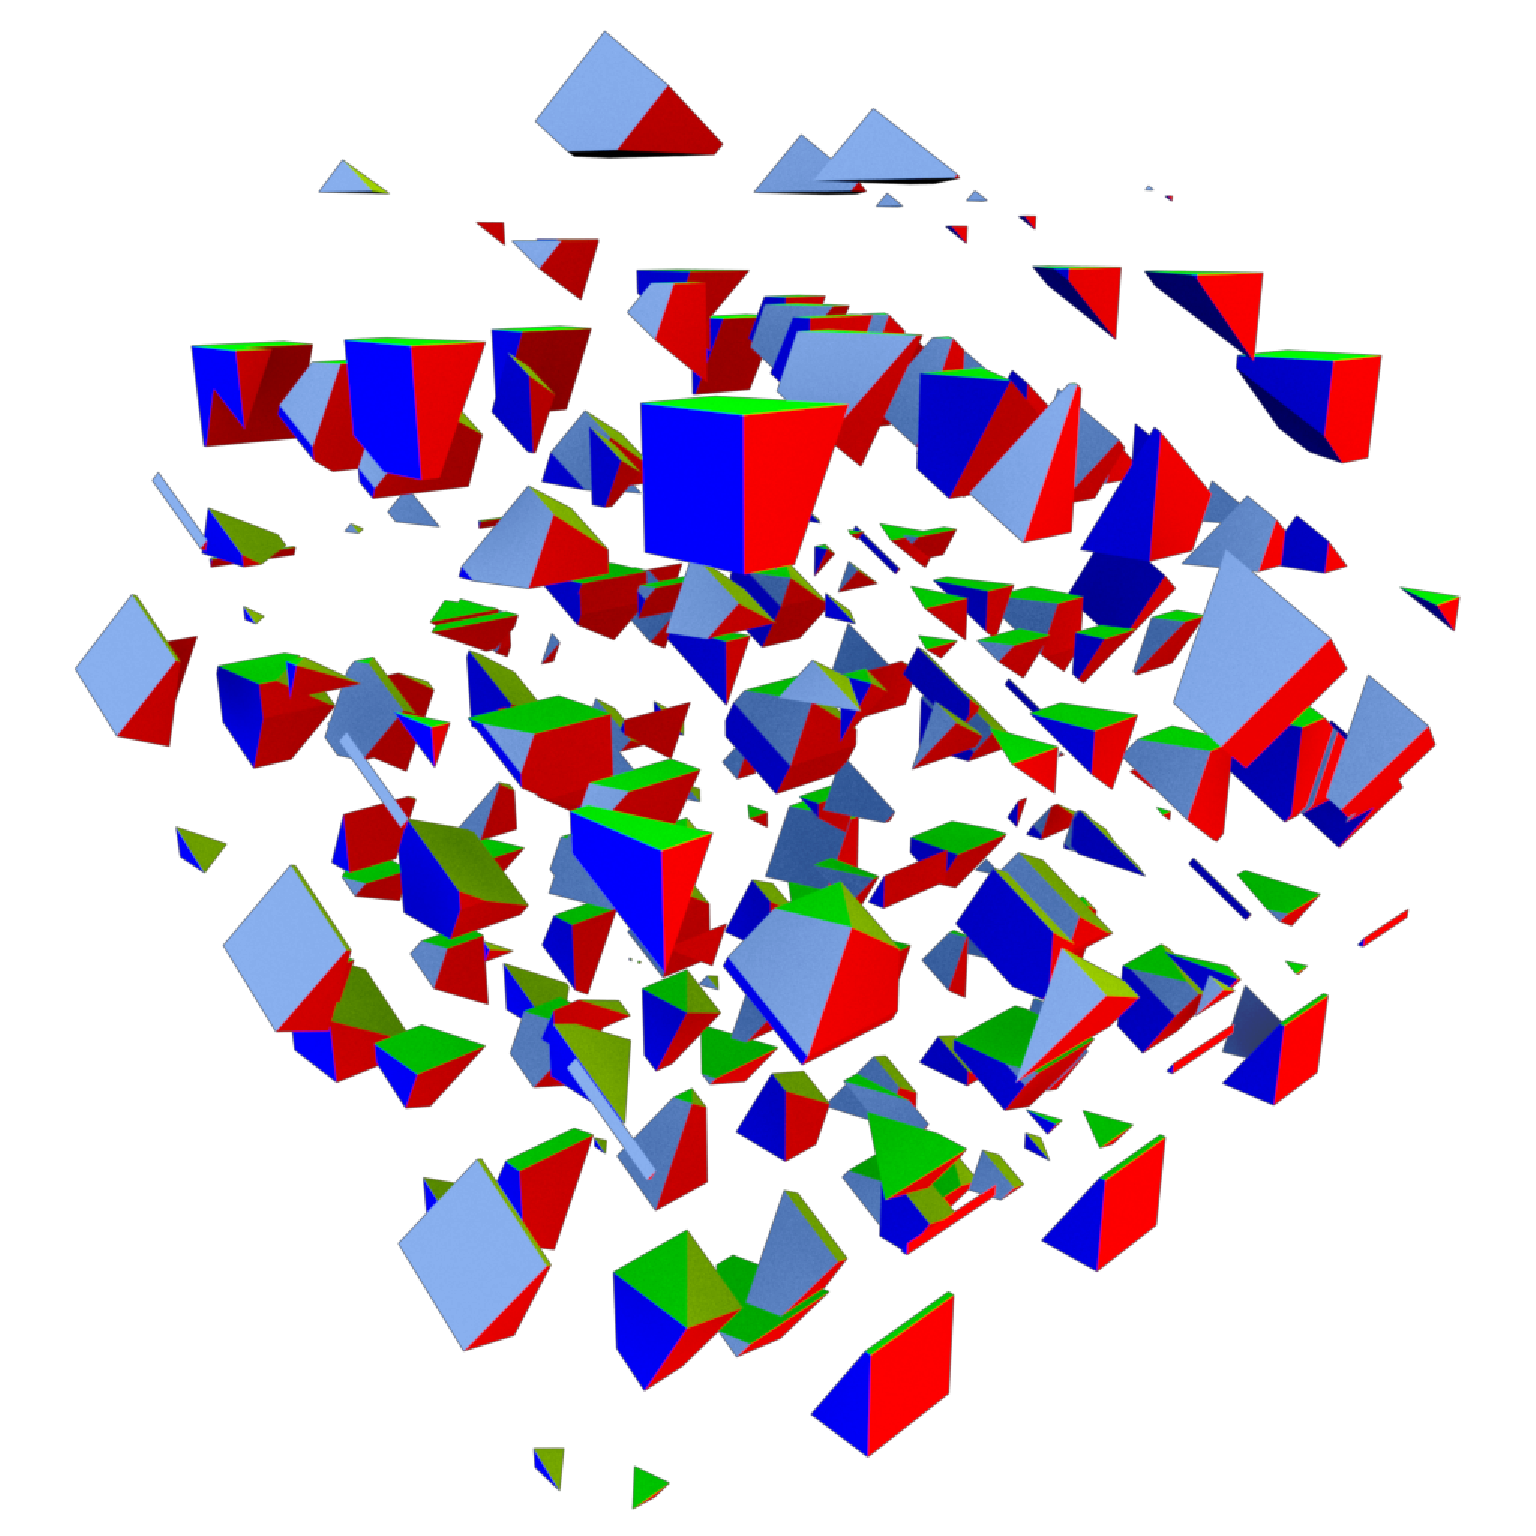
\includegraphics[width=\textwidth]{./img/test-2.pdf}%
    \caption{Output (More exploded)}
\end{figure}

